\documentclass[11pt,english]{article}
\usepackage{url}
\usepackage{graphicx}
\usepackage{hyperref}
\usepackage{amsmath}

\begin{document}
\title{Report of Problem"Latex"}
\author{Qingyu Huang}
\date{\today}
\maketitle
\thispagestyle{empty}

\newpage
\section{Error Function}
The content below is taken from Wikipdeia, the link is \url{https://en.wikipedia.org/wiki/Error_function}.
In mathematics, the error function (also called the Gauss error function) is a special function (non-elementary) of sigmoid shape that occurs in probability, statistics, and partial differential equations describing diffusion. It is defined as
\begin{equation}
erf(x)=\frac{1}{\sqrt{\pi}}\int_{-x}^x e^{-t^2} dt = \frac{2}{\sqrt{\pi}}\int_0^x e^{-t^2} dt
\end{equation}
In statistics, for nonnegative values of x, the error function has the following interpretation: for a random variable X that is normally distributed with mean $0$ and variance$1/2$, erf(x) describes the probability of X falling in the range$ [-x, x]$.

\section{The name" error function"}
The name and abbreviation for the error function(and the error function complement) were developed by J.W.L. Glaisher in 1871 on account of its connection with"the theory of Probability, and notably the theory of Errors." Glaisher cities that, for the "law of facility" of error- the normal distribution - whose density is given by
\begin{equation}
f(x)=(\frac{c}{\pi})^{1/2}e^{-cx^{2}}
\end{equation}
, the chance of an error lying between $p$ and $q$ is
\begin{equation}
(\frac{c}{\pi})^{\frac{1}{2}}\int_p^q e^{-cx^{2}} dx= frac{1}{2}(erf(q\sqrt{c})-erf(p\sqrt{c})).
\end{equation}

\begin{figure}
\centering
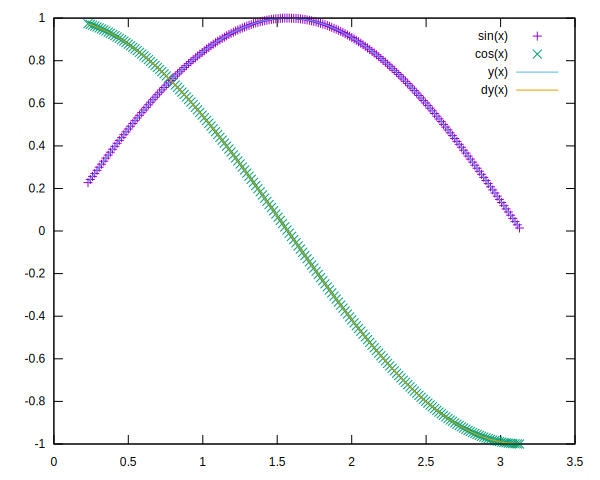
\includegraphics[width=1\linewidth]{plot}
\caption{Plot of error function erf$(x)$.}
\end{figure}
\end{document}